\section{Line Follower}
The robot utilize a line follower controller in order to navigate the factory floor. This in combination with \textbf{QR} codes and a path-planning algorithm will give a huge variety in places that the robot can be instructed to go, as long as it's on the grid and denoted with a \textbf{QR} code.

\subsection{Choice of Controller} \label{sec:choice_of_cont}

In order to move the robot to a specified point the use of a line follower controller was decided on. The robot will read in values from a camera \footnote{Refrence to the machine vision part} that publishes the angle that a \textbf{PD} controller uses as an input for calculating the signal it sends to the motors.\\
\indent The choice of a \textbf{PD} controller was made for the improved smoothness over a \textbf{P} controller and the fact that the integrating part in a \textbf{PID} controller would have undesired effects, as illustrated in Fig.\ref{fig:PID_bad}. 

\begin{figure}[H]
    \centering
    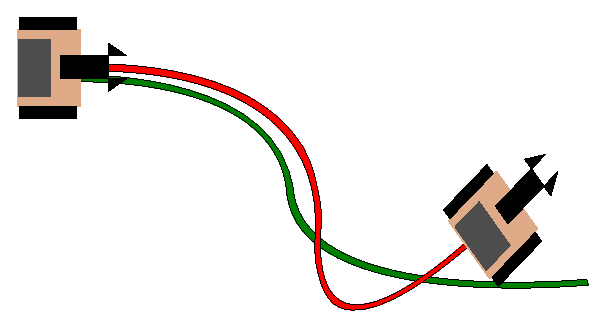
\includegraphics[width=0.7\textwidth]{img/Pid_bad.eps}
    \caption{The robot will keep acting on the integrated error even when reaching the line, this might eventually cause overshoots that makes the robot lose the line. (Green: correct path, red: actual path)  }
    \label{fig:PID_bad}
\end{figure}
